%*****************************************
\chapter{Preliminares}\label{ch:preliminares}
%*****************************************

% Sin demostraciones, solo resultados que se necesiten para secciones posteriores

Para poder comprender los resultados de los siguientes capítulos necesitaremos recordar ciertas definiciones y propiedades de álgebra que se cursan durante el grado, e introducir otros preliminares de algoritmia que formalizan el estudio. No incluiremos demostraciones, pues son los conceptos básicos de donde partiremos para desarrollar el resto del trabajo, pero el lector que quiera conocerlas puede consultar las referencias en \textbf{TODO: cite}.

\section{Preliminares de Álgebra}

% Aritmética elemental:
%	Algoritmo de Euclides: mcd
%	Congruencias
%		Ver TFG de Eva para aplicaciones de Euclides, + encontrar el inverso de a mod b con la Id de Bezout de a,b
%	Grupos y Anillos
%		Hasta grupos Z_n y sus propiedades
% 	Para el GI el grupo de las simetrías (breve)

%https://en.wikipedia.org/wiki/Schnorr_group

\paragraph{Aritmética elemental}

\begin{definition}
	Un entero $d$ se dice que es el \textbf{máximo común divisor} de dos enteros $a$ y $b$ si es el mayor entero que divide a ambos. Lo denotaremos $d=mcd(a,b)$.
\end{definition}

\hfil

Euclides describió en su obra \textit{Los Elementos} un método para calcular el $mcd$ de dos enteros, que hoy en día se conoce como \textit{Algoritmo de Euclides}. La propiedad que utiliza el algoritmo para calcular el $mcd$ es la siguiente:



\begin{proposition}
	Sean $a$, $b$ $\in \mathbb{Z}$. Entonces, para todo $\alpha \in \mathbb{Z}$ se tiene:
			\begin{center}
				$mcd(a,b) = mcd(a, b-\alpha a) = mcd(a-\alpha b, b).$
			\end{center}
	En particular, cuando $b \neq 0$ y la división entera de $a$ entre $b$ es $a = bq + r$, tenemos que $mcd(a,b) = mcd(b, r)$.
\end{proposition}

\hfil


\rule{\textwidth}{1pt}
\begin{algorithm}[Euclides]
	Encuentra el $mcd$ de $a$, $b \in \mathbb{Z}$:
	
	\begin{enumerate}
		\item Inicializa $r_0 = a$ y $r_1 = b$.
		
		\item Calcula las siguientes divisiones euclídeas
		
		\begin{tabular}{rcl}
			$r_0$ & $=$ & $q_1 r_1 + r_2$ \\
			$r_1$ & $=$ & $q_2 r_2 + r_3$ \\
			& \dots & \\
			$r_{n-3}$ & $=$ & $q_{n-2} r_{n-2} + r_{n-1}$ \\
			$r_{n-2}$ & $=$ & $q_{n-1} r_{n-1} + r_{n}$ \\
		\end{tabular}
		
		hasta que se obtenga un $r_n = 0$, con $r_{n-1} \neq 0$.
		
		\item Como $b = r_1 > r_2 > ... \geq 0$ y cada $r_i$ es entero, para $i = 1, 2, ...$, se obtiene $r_n = 0$ en un número finito de pasos y acaba el algoritmo con $mcd(a,b) = r_{n-1}$.
		
	\end{enumerate}
\end{algorithm}
\rule{\textwidth}{1pt}

\hfil

A partir del \textit{Algoritmo de Euclides} se puede expresar $d$ como una ``combinación $\mathbb{Z}$-lineal'' de $a$ y $b$:
\begin{center}
	$d = as + bt$
\end{center}
conocida como la \textit{Identidad de Bézout}.

\hfil

El algoritmo se conoce como \textit{Algoritmo de Euclides extendido}:

\rule{\textwidth}{1pt}
\begin{algorithm}[Euclides extendido]
	Encuentra el $d = mcd$ de $a$, $b \in \mathbb{Z}$ y valores $s$, $t$ $\in \mathbb{Z}$ tal que $d = as + bt$.
	\begin{enumerate}
		\item Inicializa ${\displaystyle r_{0}\gets a,r_{1}\gets b,s_{0}\gets 1,t_{0}\gets 0,s_{1}\gets 0,t_{1}\gets 1}$
		
		$i\gets 1$
		
		\item Mientras $r_i \neq 0$:
			\subitem Calcule la división euclídea $r_{i-1} = q_i r_i + r_{i+1}$
			\subitem ${\displaystyle s_{i+1}\gets s_{i-1}-q_{i}s_{i}}$
			\subitem ${\displaystyle t_{i+1}\gets t_{i-1}-q_{i}t_{i}}$
			\subitem $i \gets i+1$
		
		\item $d = r_{i-1}$	\quad	$s = s_{i-1}$ \quad  $t = t_{i-1}$
	\end{enumerate}
\end{algorithm}
\rule{\textwidth}{1pt}


\begin{remark}
	Los valores de $s$ y $t$ no tienen por qué ser únicos:
	
	${\displaystyle a(s-kb)+b(t+ka)=as-kba+bt+kba=as+bt = d}$
\end{remark}

\hfil

Utilizaremos la Identidad de Bézout para calcular los inversos en aritmética modular.

\hfil

\paragraph{Grupos y Anillos}

%TODO

\paragraph{Congruencias}

\begin{definition}
	Sean $a,\,b,\,n\,\in \mathbb{Z}$, $n \neq 0$, diremos que $a$ y $b$ son \textbf{congruentes módulo $n$}, y lo escribiremos $a \equiv b \, mod \, n$, si la diferencia $a - b$ es múltiplo de $n$.
\end{definition}

Cuando $a \equiv b \, mod \, n$ decimos que b es un \textit{\textbf{residuo} de $a$ módulo $n$}.

\begin{proposition}
	La relación de \textbf{congruencia módulo $n$} es una relación de equivalencia, es decir, es reflexiva, simétrica y transitiva.
\end{proposition}

Esto establece una relación de equivalencia en $\mathbb{Z}$, en la que la \textbf{clase} de un entero $a$ módulo $n$ es $\overline{a} = \{ a + kn \}_{k \in \mathbb{Z}}$. Cuando no exista confusión, escribiremos la clase de equivalencia $\overline{a}$ como $a$.
El correspondiente conjunto cociente, de las \textit{clases de resto módulo $n$}, es $\mathbb{Z}_n = \{\overline{0},\,\overline{1},\,\dots\overline{n-1}\}$, y hereda la suma y producto de $\mathbb{Z}$ convirtiéndose en un anillo conmutativo con neutros $\overline{0}$ para la suma y $\overline{1}$ para el producto.


\begin{theorem}
	El anillo $\mathbb{Z}_n$ es un cuerpo cuando $n$ es un número primo.
\end{theorem}

\begin{theorem}[Euler]
	Si $x$ es coprimo con 
\end{theorem}


\hfil

Si tenemos ahora dos enteros $a$ y $b$ coprimos, es decir, $mcd(a,\,b) = 1$, usando el \textit{algoritmo de Euclides extendido} podemos encontrar $r$ y $s$ de la \textit{Identidad de Bézout} tales que:
\begin{center}
	$ as + bt = 1 $
\end{center}

Si a esta igualdad le aplicamos módulo $b$, obtenemos el inverso de $a$ en $\mathbb{Z}_b$:
\begin{center}
	\begin{tabular}{ccccc}
	$  ( as + bt ) \, mod \, b $ & $\equiv $ & $as \, mod \, b $ & $ \equiv$ & $1 \, mod \, b $ \\
	$ \overline{as+bt} $ & $=$ & $\overline{as} $ & $=$ & $\overline{1} $
\end{tabular}
\end{center}

Así hemos demostrado el siguiente resultado:

\begin{proposition}
	Si $mcd(a,\,n) = 1$, entonces el elemento inverso $a^{-1}$, $0<a^{-1}<n$, existe y $a a^{-1} \equiv 1 \, mod \, n$.
\end{proposition}


\hfil

%TODO:

% Cardinal de Z^*_p
% Generador de Z^*_p, orden
% Teorema Chino de los Restos
% Pequeño teorema de Fermat o Teorema de Euler para congruencias










%
%
%
%
%
%








\section{Preliminares de Computación}

Teoría de complejidad algorítmica, problema de P NP, problema RSA de factorizar N, problemas de decisión, estadística usada en el estudio de los ZKP (\textit{ensembles}), \textit{probabilistic computations}, ...

La mayor parte está en los primeros capítulos de Fundamentals of Computer Security, y de sus referencias se podrá sacar más detallado.




%para relacionar con la criptografía, ver WIKIPEDIA
% https://en.wikipedia.org/wiki/Computational_complexity_theory#Problems_in_NP_not_known_to_be_in_P_or_NP-complete

% Handbook of applied
% Fundamentals of Computer Security
% Apuntes AED II

% Estructura:
% Intro con definiciones de problema, algoritmo, Problemas de decisión
%  Subsección: Notación asintótica, clases de complejidad (polinómico, exponencial, ejemplos)
%  Subsección: Clases P y NP, ___
%  Subsección: Algoritmos probabilísticos, ¿ensembles?, ¿preliminares de estadística?
%  Subsección: El uso en criptografía por la suposición de P!=NP, intractability, nombrar los 3 problemas NPI, y dejar el estudio y por qué son NPI para sus respectivas secciones.


En esta sección introducimos unos preliminares de complejidad computacional que nos permitirán entender de manera básica por qué se utilizan ciertos problemas matemáticos en la seguridad informática. Comencemos con unas definiciones:

\begin{definition}
	Llamamos \textit{problema} a la descripción general de una tarea que depende de unos parámetros. La \textit{definición} de un problema consta de dos partes. La primera da el escenario del problema, describiendo los parámetros necesarios. La segunda parte indica una pregunta de la que se espera una respuesta o solución.
\end{definition}

\begin{example}
	Vamos a considerar el problema de multiplicar dos matrices. La definición del problema sería:
	
	\begin{tabular}{|ll}
		\textit{Nombre:} & Problema multiplicación de matrices. \\
		\textit{Parámetros:} & Dos matrices $A_1$ y $A_2$. \\
		\textit{Pregunta:} & ¿Cuál es la matriz $A$ tal que $A=A_1 \cdot A_2$? \\
	\end{tabular}
\end{example}

\begin{definition}
   Una \textit{instancia} de un problema es el caso particular de un problema al que se le han dado valores a los parámetros.
\end{definition}


\begin{definition}	
	Un \textit{algoritmo} es una lista de instrucciones que para una instancia produce una respuesta correcta. Se dice que un algoritmo \textit{resuelve} un problema si devuelve respuestas correctas para todas las instancias del problema.
\end{definition}


\begin{definition}
	Se llama \textit{problema de decisión} a un problema cuya respuesta está en el conjunto $\mathcal{B}= \{Verdadero, Falso\}$.
\end{definition}


No todos los problemas son de decisión, pero en general es fácil transformarlos en un problema de decisión cambiando la \textit{pregunta}, y los algoritmos que resuelven un problema de decisión suelen también ser fáciles de adaptar para el problema original.

\begin{example}
	El problema del ejemplo anterior se puede transformar a un problema de decisión:
	
	\begin{tabular}{|ll}
		\textit{Nombre:} & Problema multiplicación de matrices. \\
		\textit{Parámetros:} & Tres matrices $A$, $A_1$ y $A_2$. \\
		\textit{Pregunta:} & ¿$ A = A_1 \cdot A_2$? \\
	\end{tabular}
	\\
	
	Un algoritmo para solucionarlo puede primero comprobar las dimensiones de las matrices, y si no concuerdan con las de la multiplicación, puede responder $Falso$ sin más operaciones, pero cuando las dimensiones concuerden, deberá realizar la multiplicación de $A_1$ por $A_2$ y luego comparar $A$ con el producto obtenido.
	
\end{example}

\hfil

\paragraph{Notaciones asintóticas} 

\hfil

Se utilizan para estudiar cómo crece el tiempo de ejecución, la memoria usada o cualquier otro recurso, de un algoritmo dependiendo del tamaño de los datos de entrada. Nos interesa en particular una:

\begin{definition}
	Sea $f : \mathbb{N} \rightarrow \mathbb{R}^+$. Definimos la notación \textit{O grande} u \textit{orden} de $f$ al conjunto de funciones de $\mathbb{N}$ a $\mathbb{R}^+$ acotadas superiormente por un múltiplo positivo de $f$ a partir de cierto valor $n \in \mathbb{N}$:
		
		$O(f) = \{t:\mathbb{N} \rightarrow \mathbb{R}^+ \, | \; \exists c \in \mathbb{R}^+,\, \exists 
		n_0\in \mathbb{N} \, : \, t(n) \leq c\cdot f(n) \quad \forall n \geq n_0  \}$. 

\end{definition}

\hfil

Para estudiar el tiempo de ejecución, $t : \mathbb{N} \rightarrow \mathbb{R}^+$ (el tiempo promedio, el caso más desfavorable, \dots), de un algoritmo, buscaremos una función $f$ que acote a $t$ lo más de cerca posible. Para ello definimos la relación de orden:

\begin{definition}
	Sean $f, g : \mathbb{N} \rightarrow \mathbb{R}^+$.
	\marginpar{Comparación de órdenes: $ O(1) \leq O(ln\,n) \leq O(\sqrt{n}) \leq O(n) \leq O(n\,ln\,n) \leq O(n^c) \leq O(n^{ln\,n}) \leq O(c^n) \leq O(n!) \leq O(n^n) $, donde $c>1$ constante.}
	Diremos que  $O(f) \leq O(g)$ si $\forall t \in O(f)$ se tiene que $t \in O(g)$, es decir,  $O(f) \subseteq O(g)$.
\end{definition}

Para acotar $t$ buscaremos el menor $O(f) : t\in O(f)$.

% La función $t : \mathbb{N} \rightarrow \mathbb{R}^+$, del tiempo de ejecución de un algoritmo, toma en general como parámetro el tamaño de la entrada. Éste depende de la representación que se le dé a los parámetros, pero podemos pensar siempre en la representación binaria de los números enteros excepto que se indique lo contrario. Esta representación utiliza $1+log_2(n)$ bits para un entero $n$, y podemos simplificar para $n$ suficientemente grande a $log_2(n)$.

\hfil 

\paragraph{Clases de complejidad}

\hfil

 Para estudiar los problemas de decisión los organizamos en clases de complejidad, según sus mejores algoritmos que los solucionan.


\begin{definition}
	Se llama algoritmo de \textit{tiempo de cálculo polinomial} al algoritmo cuya función de tiempo del caso más desfavorable es de orden $O(n^k)$, donde $n$ es el tamaño de la entrada y $k$ una constante. Cualquier algoritmo cuyo tiempo de ejecución no puede acotarse de esa manera se llama de \textit{tiempo de cálculo exponencial}.
\end{definition}

A veces se denominan \textit{buenos} o \textit{eficientes} a los algoritmos polinomiales, e \textit{ineficientes} a los exponenciales. Sin embargo, hay casos particulares donde no ocurre. Lo más importante al tratar con algoritmos polinomiales es el grado del polinomio, $k$, que indica su orden de complejidad. Por ejemplo, consideremos un problema cuyo mejor algoritmo tarda $n^{100}$ instrucciones, es de orden polinómico, pero prácticamente intratable a partir de $n=2$, y por otra parte, un problema que utilice $2^{0.00001n}$ instrucciones podría tratar casos hasta de $n=10^6$ sin dificultad.
Por esto, en criptografía se debe considerar el caso promedio sobre el caso más desfavorable.


\begin{definition}
	El conjunto de problemas de decisión que se pueden resolver en tiempo polinomial se llama clase \textbf{P}.
\end{definition}

\begin{definition}
	Se llama clase de complejidad \textbf{NP} al conjunto de problemas de decisión donde una respuesta que sea $Verdadero$ se puede verificar en tiempo polinomial, dada cierta información extra, que llamaremos \textit{certificado}.
	\label{def:NP}
\end{definition}

\begin{definition}
	Se llama clase de complejidad \textbf{co-NP} al conjunto de problemas de decisión donde una respuesta que sea $Falso$ se puede verificar en tiempo polinomial, dado el correspondiente \textit{certificado}.
\end{definition}

Es inmediato que  que \textbf{P} $\subseteq$ \textbf{NP} y \textbf{P} $\subseteq$ \textbf{co-NP}.

\begin{example}[Problema en \textbf{NP}]
	Consideremos el siguiente problema de decisión:
	
		\begin{tabular}{|ll}
		\textit{Nombre:} & Problema del entero compuesto. \\
		\textit{Parámetros:} & Un entero positivo $n$. \\
		\textit{Pregunta:} & ¿Es $n$ compuesto? Es decir, ¿existen \\
			&  enteros $a$, $b > 1$ tal que $n=ab$? \\
	\end{tabular}
	\\
	
	El problema pertenece a \textbf{NP} porque se puede comprobar en tiempo polinomial que $n$ es compuesto si nos dan su \textit{certificado}, un divisor $a$ de $n$, tal que $1 < a < n$. Basta usar la división euclídea de $n$ entre $a$ y ver que el resto es $0$. Sin embargo, aún no se conoce si pertenece a \textbf{P}.
\end{example}


\hfil

\begin{definition}
	Sean dos problemas de decisión $L_1, L_2 \in $ \textbf{NP}, con correspondientes conjuntos de instancias $I_1$ e $I_2$. Sean $I_1^+$ e $I_2^+$ los subconjuntos de todas las instancias ``$Verdaderas$'' de $I_1$ e $I_2$, respectivamente. Decimos que $L_1$ es \textit{reducible en tiempo polinomial} a $L_2$, $L_1 \leq_P L_2$, si existe una función $f:I_1 \Rightarrow I_2$ que cumple:
	
	\begin{enumerate}
		\item Es ejecutable en tiempo polinomial.
		\item $x \in I_1^+  \Leftrightarrow  f(x) \in I_2^+ $.
	\end{enumerate}
\end{definition}

\hfil

De manera más informal, si $L_1 \leq_P L_2$, entonces $L_2$ es computacionalmente tan difícil como $L_1$, o de otro modo, $L_1$ no es más difícil que $L_2$.

\begin{definition}
	Un problema de decisión $L$ se dice que es \textbf{NP}-completo, o \textbf{NPC} si:
	\begin{enumerate}[label=(\roman*)]
		\item $L \in $ \textbf{NP}, y
		\item $L_1 \leq_P L \quad \forall L_1 \in $ \textbf{NP}.
	\end{enumerate}
\end{definition}

\hfil

Los problemas \textbf{NPC} son los más difíciles entre los \textbf{NP} en el sentido de que son al menos tan difíciles como el resto de problemas en \textbf{NP}. Veamos el problema \textbf{NPC} más característico:

	\begin{tabular}{|ll}
		\textit{Nombre:} & Problema de satisfacibilidad booleana (SAT). \\
		\textit{Parámetros:} & Una colección finita $C$ de expresiones booleanas \\
				 &  con variables y sin cuantificadores. \\
		\textit{Pregunta:} & ¿Hay alguna asignación de las variables que \\ & haga $Verdadero$ a $C$? \\
	\end{tabular}
	\\

\begin{theorem}[Teorema de Cook (1971)]
	El problema de satisfacibilidad booleana es \textbf{NPC}.
\end{theorem}\marginpar{Para conocer más sobre el problema y la demostración se puede consultar \citep{book:1056906}.}


O expresado de otra manera:

\begin{theorem}
	Todo problema $Q \in $ \textbf{NP} se puede reducir en tiempo polinomial al problema de satisfacibilidad booleana.
	
	$\forall Q \in $ \textbf{NP}, $Q \leq_P SAT$.
\end{theorem}


\hfil

A día de hoy conocemos ciertas propiedades sobre las clases de equivalencia, pero quedan muchas cuestiones sin resolver:

\begin{itemize}
	\item Uno de los siete problemas del milenio, ¿\textbf{P} $=$ \textbf{NP}?
	\item ¿\textbf{NP} $=$ \textbf{co-NP}?
	\item ¿\textbf{P} $=$ \textbf{NP} $\cap$ \textbf{co-NP}?
\end{itemize}


La opinión de los expertos en base a ciertas evidencias es que la respuesta a las tres es NO, pero hasta que se encuentren demostraciones formales de cada una, quedarán en conjeturas. Y basándose en esas conjeturas es donde se apoya la seguridad informática.


\begin{figure}[bth]
	\begin{center}
		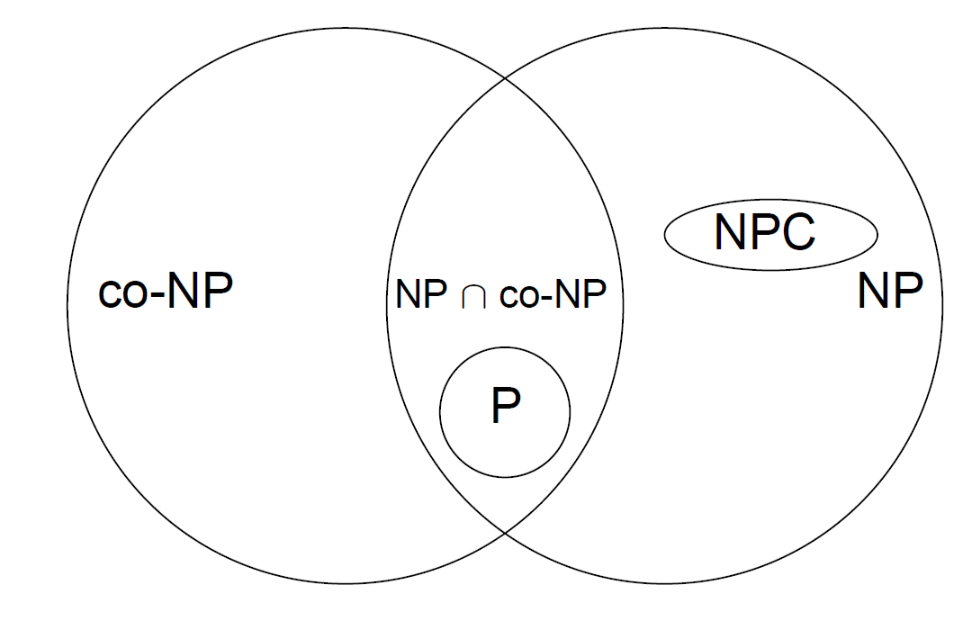
\includegraphics[width=.45\linewidth]{gfx/NPclasses}
	\end{center}
	\caption{Conjetura de las relaciones entre clases \textbf{NP}, \textbf{co-NP}, \textbf{NPC}, \textbf{P}.}
	\label{fig:NPclasses}
\end{figure}


Existen tres problemas que se conoce que pertenecen a \textbf{NP}, pero se desconoce a día de hoy si pertenecen a \textbf{P} o \textbf{NPC}: el isomorfismo de grafos, el logaritmo discreto y la factorización de enteros.

En los siguientes capítulos los estudiaremos como base de diferentes pruebas de conocimiento cero.


\hfil


\paragraph{Algoritmos probabilísticos} 

\hfil

Para intentar resolver la infactibilidad computacional de ciertos problemas, surge un modelo alternativo de computación que utiliza métodos probabilísticos. Estos métodos no pueden asegurar cotas superiores absolutas de tiempo, e incluso pueden devolver una respuesta errónea. Sin embargo, dadas unas cotas muy pequeñas de errores, en la práctica, ciertos métodos probabilísticos son más eficientes que los algoritmos conocidos, pues el tiempo de ejecución \textit{esperado} del método, calculado probabilísticamente, es menor que el orden del algoritmo original.


% Tipos de algoritmos probabilísticos según errores
% Ejemplo de test de primalidad

\begin{definition}
	Llamamos \textit{algoritmo de Monte Carlo} a un algoritmo probabilístico que resuelve un problema de decisión, pero tiene un error $\epsilon$ de equivocarse.
	
	Decimos que es \textit{parcialmente} $Verdadero$ si cuando se le da una instancia $Verdadera$ nunca se equivoca, pero si la instancia es $Falsa$ puede devolver $Verdadero$ con probabilidad $\epsilon$. De la misma manera, decimos que es \textit{parcialmente} $Falso$ si siempre resuelve correctamente instancias $Falsas$, pero puede cometer un error al resolver instancias $Verdaderas$.
\end{definition}


\begin{definition}
	Llamamos \textit{algoritmo de Las Vegas} a un algoritmo probabilístico que resuelve un problema de decisión, pero o bien lo resuelve correctamente, o bien informa de error y termina sin resolver el problema con una probabilidad $\epsilon$.
\end{definition}



\begin{example}[Test de primalidad]
	El problema de decisión
	
	\begin{tabular}{|ll}
		\textit{Nombre:} & Problema de primalidad (PRIM). \\
		\textit{Parámetros:} & Un entero $n$. \\
		\textit{Pregunta:} & ¿Es $n$ primo? \\
	\end{tabular}
	\\
	es un problema en \textbf{NP}$\cap$\textbf{co-NP} (es el contrario del problema del entero compuesto), pero no se conoce ningún algoritmo que lo resuelva en tiempo polinómico, por ello no sabemos aún si pertenece a \textbf{P}.
	
	Un algoritmo probabilístico basado en el Pequeño Teorema de Fermat, $a^{n-1} \equiv 1 \, mod \, n$ si $n$ es primo para cualquier $a\in \mathbb{Z}_n$, puede utilizarse para comprobar si $n$ es primo.
	
	Si $n$ es primo, para todo $a$ que se elija, se cumplirá $a^{n-1} \equiv 1 \, mod \, n$, por lo que es un algoritmo de Monte Carlo parcialmente $Verdadero$, para una instancia $Verdadera$ nunca se equivoca.
	
	Sin embargo, si $n$ es compuesto, pueden existir valores $a$ que cumplan la propiedad. Por ejemplo, si $n$ es un \textit{número de Carmichael}, todo $a$ coprimo con $n$ cumple $a^{n-1} \equiv 1 \, mod \, n$.
	
	Este no es el test de primalidad más fuerte, existen otros mejorados, como el test de primalidad de Miller-Rabin, que asegura que a lo sumo da un falso positivo para $\frac{1}{4}$ de todos los enteros $a$, $0<a\leq p-1$. Ejecutando el test un número $k$ de veces, eligiendo aleatoriamente $a\in \mathbb{Z}_n$, obtenemos una probabilidad de error de $\epsilon=\frac{1}{4^k}$, lo que podría darnos en 50 iteraciones un algoritmo ejecutable en tiempo polinomial, con probabilidad de error, cuando $n$ es compuesto, de $2^{-50}$, algo que podemos estar dispuestos a asumir en la práctica.
	
\end{example}






%
%
%
%
%
%






\section{Preliminares de Probabilidad}



% JL Gomez Pardo Introduction to cryptography with Mapple
% Elementos probabilidad Zoroa
% Fundamentals
% https://en.wikipedia.org/wiki/Computational_indistinguishability

%% Depende de si pongo computacionalmente indistinguible, y en el capítulo de ZKP da un resumen de lo que es por límites, más una línea informal, sobra.


%
%
%
%
%
%




\section{Preliminares de Grafos}

% Si ponemos GI y a lo mejor lo pasamos al capítulo correspondiente.
